\cleardoublepage % memastikan bab baru dimulai di halaman ganjil (kanan)

\chapter{STUDI LITERATUR}
\label{chap:studi-literatur}

Bagian ini memberikan penjelasan mendalam serta gambaran terkait sumber daya yang digunakan dalam mengerjakan tugas akhir ini. Sumber daya tersebut setidaknya mencakup beberapa hal, namun tidak terbatas pada model, parameter, data, prosedur \textit{fine-tuning}, serta metode analisis. Tiap cakupan disusun untuk mendukung latar belakang, rumusan masalah dan hipotesis, serta menegaskan celah riset sebagaimana telah dibahas di Bab \ref{chap:pendahuluan}. Oleh karena itu, bagian ini diharapkan dapat mempermudah pemahaman definisi tiap sumber daya secara sistematis dan menyeluruh.

\section{Pengetahuan Kasus}
\label{chap:sl_ptk}

\subsection{Pemahaman Semantik pada LLM dan Keterbatasannya}
\label{sub:sl_semantik}

Pemahaman semantik merujuk pada kemampuan model menangkap makna suatu teks, bukan sekadar menemukan pola kemunculan kata. Pada LLM, model dilatih dengan objektif prediksi kata berikutnya (\textit{next-word-prediction}) sehingga representasinya terbentuk dari kalkulasi statistik teks, misalnya frekuensi atau panjang kata. Pelatihan ini menghasilkan kemampuan bahasa yang kuat, tetapi tidak menjamin bahwa representasi internalnya menyerupai bagaimana manusia memproses makna. 

\textcite{mahowald2024dissociating} membedakan kompetensi linguistik formal (aturan dan pola bahasa) dari kompetensi fungsional (penalaran dan penggunaan bahasa di dunia nyata), dan menunjukkan bahwa LLM jauh lebih andal pada kompetensi yang pertama. Selain itu, \textcite{yu2024predicting} juga mengutarakan bahwa prediksi kata tidak mencerminkan pemrosesan berlapis pada LLM. Apakah LLM benar-benar memahami makna atau hanya meniru pola statistik juga masih diperdebatkan \autocite{mitchell2023debate}. Keterbatasan semacam inilah yang melatarbelakangi riset \textcite{moussa2025improving}, yang menerapkan \textit{brain-tuning} pada model ucapan dengan pemahaman semantik rendah (Wav2vec2.0, HuBERT, serta Whisper) untuk memperbaikinya. Dengan demikian, fokus utama pengembangan terletak pada bagaimana meningkatkan pemahaman semantik pada representasi internal LLM, namun kemampuan umum atau fungsionalitasnya dalam mendeteksi pola yang sudah kuat tetap terjaga.

Pemahaman semantik tidak dapat diamati langsung, sehingga diukur secara tidak langsung, yaitu melalui kinerja pada tugas hilir (\textit{downstream task}) (Subbab \ref{sub:sl_evaluasi}) dan melalui keselarasan representasi dengan aktivitas otak manusia (Subbab \ref{sub:sl_encoding}). Hal tersebut memunculkan pertanyaan yang mendasari penelitian ini, yaitu apakah sinyal otak sebagai sumber informasi nonteks dapat memperbaiki representasi LLM.

\subsection{Pemrosesan Bahasa di Otak}
\label{sub:sl_otak}

Otak memproses bahasa lisan secara bertahap. Bahasa diterima dalam bentuk sinyal suara oleh koklea dan batang otak untuk diteruskan ke nukleus genikulatum medial (MGN) di talamus, lalu diproyeksikan ke korteks auditori primer \autocite{hamilton2021parallel}. 
Proses tersebut berfungsi untuk mengkodekan suara (sinyal akustik) menjadi informasi berkategori fonem (vokal dan konsonan) serta memetakan fitur artikulasi vokal secara meluas ke area yang lebih jauh di korteks \autocite{deheer2017hierarchical}. \textcite{mischler2024contextual} menuturkan bahwa informasi yang diproses area tersebut merepresentasikan informasi yang lebih abstrak, termasuk yang lebih kontekstual. Informasi ini merupakan informasi makna atau semantik yang tidak terpusat pada satu area. \textcite{huth2016natural} memetakan respons fMRI partisipan dan menemukan bahwa representasi makna tersebut tersebar luas di korteks. Pada taraf kalimat, makna proposisional juga dikodekan oleh jaringan korteks terdistribusi \autocite{anderson2021deep}. Secara hierarkis, pemrosesan bahasa di otak melibatkan kinerja sinergis antararea korteks untuk menerjemahkan sinyal suara menjadi pemahaman bahasa yang padu. 

Secara harfiah, "area yang lebih jauh" didefinisikan sebagai area korteks yang lebih dalam dari korteks auditori primer dengan tujuan khusus dalam memproses bahasa. Secara urut, area yang pertama kali memproses bahasa pada area tersebut adalah sulkus temporal superior (STS) \autocite{deheer2017hierarchical}. Pada area ini, fonem hasil pengkodean suara yang berhasil dikenali STS akan didistribusikan melalui dua alur: (1) alur ventral pada girus temporal tengah/bawah (MTG/ITG) dan lobus temporal anterior (ATL) untuk pemetaan bentuk bunyi kata dengan makna, serta (2) alur dorsal pada sylvian parietal-temporal (Spt) dan korteks premotor frontal untuk pemetaan persepsi bunyi ke perintah motorik artikulasi ucapan \autocite{saur2008langpathways}. Selanjutnya, informasi dari kedua alur tersebut bermuara pada korteks frontal tingkat tinggi untuk integrasi bahasa yang lebih kompleks. Girus frontal bawah (IFG) menjadi pusat dalam tahapan ini, di mana pars opercularis (BA 44) mengolah struktur sintaksis hierarkis yang rumit, sedangkan pars triangularis (BA 45) mengelola seleksi makna dan pemecahan ambiguitas semantik. Selain itu, korteks prefrontal dorsolateral (DLPFC) juga berkontribusi dalam mendukung memori kerja fonologis dan kontrol eksekutif untuk memahami struktur kalimat panjang atau ambigu \autocite{friederici2011brain}.

Apabila diperhatikan, pemrosesan bahasa di otak manusia terjadi terutama pada jaringan frontal dan temporal (frontotemporal). Pemrosesan bahasa bergantung pada jaringan tersebut yang dapat ditentukan secara fungsional pada setiap individu \autocite{fedorenko2010new}. Namun, interaksi antara kedua jaringan ini berbeda dari sistem \textit{multiple-demand} (MD) yang bertanggung jawab atas kontrol kognitif, pemecahan masalah, serta pengorganisasian langkah-langkah tugas (\textit{mental programs}) \autocite{duncan2010multiple}. Lebih lanjut, \textcite{fedorenko2024language} menuturkan bahwa bahasa dipandang terutama sebagai alat komunikasi, bukan alat untuk berpikir. Perbedaan pandangan fungsi bahasa ini penting dianalisis karena pada dasarnya sinyal otak dari jaringan bahasa belum tentu relevan terhadap kemampuan nonlinguistik atau kognitif model.

Selain itu, otak secara aktif memprediksi kata yang akan muncul. \textcite{goldstein2022shared} merekam respons otak partisipan dengan ECoG saat mendengar siniar dan menemukan fakta bahwa otak memuat informasi prediktif akan kata berikutnya sebelum kata tersebut terucapkan, serupa dengan objektif LLM. Kesamaan prinsip ini membuat perbandingan antara representasi LLM dan aktivitas otak lebih bermakna. % VERIFIKASI: rincian metode, angka korelasi, dan jendela waktu prediksi dari Goldstein dkk. sebelum dicantumkan

\subsection{Data fMRI Naturalistik}
\label{sub:sl_naturalistik}

Pada data naturalistik, partisipan mendengarkan atau membaca cerita utuh sehingga konteks terjaga, serupa dengan konteks yang diproses LLM. Konsekuensinya, sinyal otak yang terekam bercampur dengan banyak fitur linguistik dan nonlinguistik, sehingga dibutuhkan data dalam jumlah besar per partisipan (Subbab \ref{sub:sl_fmri}). Riset ini menggunakan dataset fMRI naturalistik \autocite{lebel2023natural} sebagai sumber utama sinyal otak untuk \textit{brain-tuning}, serta \textit{Narratives} \autocite{nastase2021narratives} untuk menguji generalisasi lintas dataset yang digunakan secara opsional pada tahap evaluasi akhir. % TODO: isi spesifikasi singkat kedua dataset (partisipan, stimulus, TR); detail teknis sudah di Subbab \ref{sub:sl_fmri}

Dataset \textcite{lebel2023natural} menyajikan rekaman respons BOLD fMRI dari otak manusia saat mendengarkan narasi. Dataset ini memetakan fitur bahasa seperti fonem, laju kata, dan makna semantik terhadap aktivitas korteks otak. Selain data mentah fMRI, data ini juga dilengkapi oleh turunan data fMRI yang telah dipraproses, rekonstruksi permukaan korteks 3D, transkrip audio, dan pustaka \textit{Python} untuk pemodelan. Di sisi lain, Narratives \autocite{nastase2021narratives} merupakan dataset berformat BIDS dan dilengkapi transkrip terdeteksi hingga skala kata dan fonem yang berfungsi sebagai \textit{benchmark} terbuka untuk mengevaluasi model komputasi pemahaman bahasa pada otak manusia. Spesifikasi dataset Narratives tidak dijelaskan secara eksplisit baik dalam tabel ataupun penjelasan tekstual karena pengaplikasiannya bersifat opsional hanya jika waktu pengerjaan masih tersedia. Secara lengkap, tersaji Tabel \ref{tab:sl_naturalistik} yang berisi daftar  singkat spesifikasi data fMRI \autocite{lebel2023natural}.

\input tables/speklebel.tex

Pemanfaatan dataset fMRI yang dipadukan dengan LLM dilakukan pada riset milik \textcite{Tang2023858} untuk merekonstruksi teks kontinu secara langsung dari representasi semantik di korteks otak. Penggabungan model enkoding semantik, model bahasa generatif, dan algoritma \textit{beam search} dalam sebuah dekoder, terbukti berhasil mengatasi keterbatasan resolusi temporal sinyal BOLD fMRI. Dekoder tersebut tidak hanya menerjemahkan ucapan tetapi juga \textit{imagined speech} dan deskripsi teks. Riset tersebut menjadi validasi kebermanfaatan dataset fMRI naturalistik pada LLM.

\section{Landasan Teori}
\label{chap:sl_ldt}

\subsection{Model Bahasa Besar dan Transformer}
\label{sub:sl_llm}
Model bahasa besar atau \textit{Large Language Model} (LLM) merupakan salah satu kategori model pembelajaran mendalam (\textit{deep learning}) yang menerapkan kombinasi antara arsitektur koneksionis, \textit{Big Data}, dan algoritma pembelajaran mesin (\textit{machine learning}) \autocite{nefdt2026s}. LLM dibangun dengan basis arsitektur jaringan saraf buatan yang disebut \textit{transformer}. Arsitektur tersebut terdiri atas jaringan saraf (\textit{neuron}) multilapis yang saling terhubung melalui miliaran bobot (\textit{weight}) atau parameter. Berbeda dengan arsitektur model \textit{deep learning} lainnya, \textit{transformer} mengolah rentetan (\textit{sequence}) teks/kata dan mengidentifikasi pola yang terdapat di dalamnya. Pengidentifikasian pola tersebut memiliki tujuan untuk memprediksi teks/kata yang akan muncul berikutnya berdasarkan rentetan teks/kata sebelumnya \autocite{Stryker_2024}.

Lebih lanjut, \textcite{Stryker_2024} juga memaparkan bahwa pada LLM, data teks/kata dilatih dengan teknik \textit{self-supervised learning}. Teknik ini mengoptimalisasi kinerja dengan basis \textit{ground-truth} (prediksi keluaran yang "benar" dari masukan tertentu) tanpa pelabelan data. Data teks/kata masukan diurai menjadi kumpulan token melalui proses \textit{tokenization} yang menstandardisasi bahasa sehingga dapat ditangani secara konsisten. LLM memproses token pada jaringan \textit{transformer} melalui mekanisme \textit{self-attention}. Mekanisme ini merupakan komponen inti arsitektur \textit{transformer} yang berperan untuk memperkaya pemahaman model dengan relasi antarelemen rentetan data \autocite{app14104316}. Mekanisme tersebut diilustrasikan pada Gambar \ref{fig:attention}.

\begin{figure}[h] % pilihan opsi yang disarankan: t = top, b = bottom, h = here
  \centering
  \caption{Mekanisme \textit{self-attention} pada \textit{Transformer} \autocite{app14104316}} 
	\label{fig:attention}
    	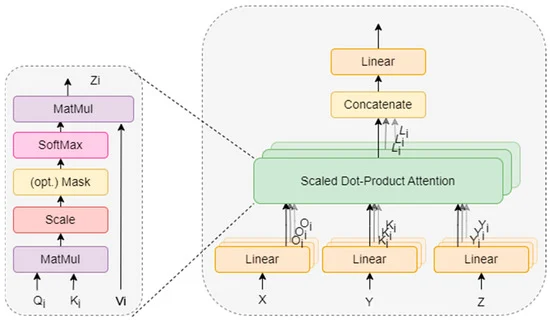
\includegraphics[width=0.7\textwidth]{images/attention.png}
\end{figure}

Mekanisme \textit{self-attention} pada Gambar \ref{fig:attention} menjelaskan bahwa pada sisi kiri, proses \textit{scaled dot-product attention} dijabarkan sebagai komponen inti dari serangkaian proses \textit{multi-head attention} pada sisi kanan. Pada mekanisme ini, input yang berupa matriks \textit{query} $Q$ di-\textit{dot-product} dengan matriks \textit{key} $K$. Hasil tersebut kemudian dinormalisasi untuk menjaga stabilitas gradien berupa probabilitas $P$. Selanjutnya, dikenakan fungsi aktivasi $Softmax(P)$ yang di-\textit{dot-product} dengan matriks \textit{value} $V$, dimana vektor dengan $P$ terbesar diberi atensi (\textit{attention}) lebih banyak pada lapisan berikutnya. Mekanisme ini dijabarkan secara komprehensif di Persamaan \ref{eq:attention}. 

\begin{equation}
  Attention(Q,K,V) = Softmax\left(\frac{Q\cdot{K^T}}{\sqrt{d_k}}\right)\cdot{V}
  \label{eq:attention}
\end{equation}
\eqcaption{Persamaan Attention}

Pada \textit{multi-head attention}, $Q$, $K$, dan $V$ diproyeksikan secara linear sebanyak $h$ kali menggunakan bobot yang berbeda-beda. Setiap proyeksi (\textit{head}) menghitung atensi secara paralel dengan Persamaan \ref{eq:attention}, lalu seluruh outputnya digabungkan (\textit{concatenate}) dan diproyeksikan kembali dengan $W^O$ seperti pada Persamaan \ref{eq:multihead}.

\begin{equation}
  \begin{gathered}
    MultiHead(Q,K,V) = Concat(head_1, \ldots, head_h)\, W^O \\
    \text{di mana } head_i = Attention(Q W_i^Q,\, K W_i^K,\, V W_i^V)
    \label{eq:multihead}
  \end{gathered}
\end{equation}
\eqcaption{Persamaan \textit{Multi-Head Attention}}

Lebih lanjut, arsitektur \textit{transformer} tersusun atas dua struktur, yakni \textit{encoder} dan \textit{decoder}. \textcite{vaswani2017attention} menjelaskan bahwa \textit{encoder} berfungsi memetakan rentetan masukan berupa representasi simbol $(x_1, \ldots, x_n)$ ke rentetan representasi kontinu $z = (z_1, \ldots, z_n)$. \textit{Encoder} terdiri atas $N$ tumpukan (\textit{stack}) yang tiap tumpukannya diisi dua sublapisan. Sublapisan pertama menerapkan mekanisme \textit{multi-head attention}, dan sublapisan kedua merupakan jaringan \textit{feed-forward} terhubung penuh (\textit{fully-connected}), sederhana, dan berbasis posisi. Setelah itu, \textit{decoder} akan menghasilkan rentetan $y = (y_1, \ldots, y_m)$ berupa simbol satu per satu. \textit{Decoder} terdiri atas $N$ tumpukan yang diisi tiga sublapisan. Dua di antaranya serupa dengan \textit{encoder} (\textit{multi-head attention} dan \textit{feed-forward}), ditambah satu sublapisan yang memproses luaran \textit{encoder} via \textit{multi-head attention}. Pada riset ini, digunakan model \textit{decoder-only} dengan atensi kausal yang umum pada kebanyakan LLM modern.

\subsection{Prosedur {Fine-Tuning} dan Mekanisme LoRA}
\label{sub:sl_finetuning}
 
Pelatihan LLM umumnya terdiri atas dua tahap. Tahap pertama adalah \textit{pretraining} pada korpus teks berskala besar dengan tugas \textit{next-word-prediction} untuk memperoleh representasi bahasa yang general. Tahap kedua adalah \textit{fine-tuning}, yang melanjutkan pelatihan model dengan data yang lebih kecil dan fungsi \textit{loss} yang sesuai. Pada \textit{full fine-tuning}, seluruh parameter diperbarui melalui \textit{gradient descent} terhadap fungsi \textit{loss}. Pendekatan ini digunakan oleh \textcite{negi2025brain} yang memperbarui seluruh parameter LLM (BERT dan mBERT) dengan sinyal fMRI sebagai target untuk meningkatkan pemahaman multibahasa. % VERIFIKASI: model dasar (BERT atau varian multibahasa) dan cakupan lapis yang diperbarui
Hal ini masih dapat dilakukan karena BERT berparameter jutaan. Pada model berparameter miliaran, \textit{full fine-tuning} membutuhkan memori yang besar dan berisiko membuat model melupakan kemampuan awalnya (\textit{catastrophic forgetting}). Risiko tersebut dapat didefinisikan sebagai penurunan fungsionalitas model saat keselarasan mungkin mengalami peningkatan.
 
\textit{Low-Rank Adaptation} (LoRA) \autocite{hu2022lora} mengatasi masalah tersebut dengan membekukan matriks bobot \textit{pretraining} $W_{0 (d \times k)}$ dan hanya melatih pembaruan bobot \textit{rank} rendah $\Delta W = BA$, dengan $B_{(d \times r)}$, $A_{(r \times k)}$, dan $r < \min(d,k)$. Bobot baru serta target luaran diperoleh melalui Persamaan \ref{eq:lora}, dengan $\frac{\alpha}{r}$ sebagai faktor skala.
 
\begin{equation}
  L = W_{\text{baru}} \cdot x ;\; W_{\text{baru}} = W_0 + \frac{\alpha}{r}\ B \cdot A
  \label{eq:lora}
\end{equation}
\eqcaption{Persamaan \textit{Low-Rank Adaptation} (LoRA)}
 
Matriks $B$ diinisialisasi dengan nol sehingga pada awal pelatihan $\Delta W = 0$ dan perilaku model identik dengan model \textit{pretrained}. Jumlah parameter yang dilatih  turun dari $d \times k$ menjadi $r(d+k)$. LoRA umumnya dipasang pada matriks proyeksi atensi ($W^Q$, $W^K$, $W^V$, dan $W^O$) sebagaimana telah dijelaskan pada Persamaan \ref{eq:multihead}.

Selain LoRA terdapat QLoRA (\text{Quantized Low-Rank Adaptation}) \autocite{dettmers2023qloraefficientfinetuningquantized} yang digunakan secara opsional pada riset ini untuk model berparameter 4--8 miliar. QLoRA mengatasi keterbatasan LoRA yang membutuhkan banyak memori pada jumlah parameter yang jauh lebih besar. Hal ini dikarenakan LoRA beroperasi pada taraf memori 16-bits. QLoRA hadir dengan kuantisasi pembekuan bobot \textit{pretraining} $W_{0}$ menjadi 4-bits untuk selanjutnya dilatih pada adapter LoRA. Pendekatan ini terbukti efektif dalam \textit{fine-tuning} LLM parameter 65B pada GPU tunggal.

Dalam konteks \textit{brain-tuning}, \textit{tuning} dengan atau tanpa LoRA telah digunakan. \textcite{xiao2026beyond} menerapkan LoRA pada modul atensi di lapis tengah untuk menggabungkan objektif sinyal otak dengan label bahasa pada model berukuran 1,5B hingga 72B parameter demi penalaran yang lebih kokoh, sedangkan \textcite{negi2025brain} memakai \textit{full fine-tuning} pada model kecil (BERT) berparameter kurang dari miliaran. % TODO: tegaskan pilihan yang dipakai pada penelitian ini (LoRA atau full fine-tuning), beserta alasan dan nilai rank $r$
 
 
\subsection{Dataset fMRI Naturalistik dan Sinyal BOLD}
\label{sub:sl_fmri}
 
\textit{Functional Magnetic Resonance Imaging} (fMRI) merekam aktivitas otak secara tidak langsung melalui sinyal \textit{blood-oxygen-level-dependent} (BOLD), yaitu perubahan kadar oksigen darah yang menyertai aktivitas neuron. Prosedur perekaman tersebut dengan menyimpan 27 audio cerita 
siniar \textit{The Moth}. Dari audio tersebut, diekstrak tiga fitur bahasa: \textit{Semantic Feature} (makna kata), \textit{Phoneme Feature} (bunyi bahasa), dan \textit{Word Rate Feature} (laju kata per detik) yang dipetakan terhadap waktu.

Cerita pada siniar dibawakan dengan laju pembicaraan yang cepat (beberapa kata per detik). Hal ini berlawanan dengan prosedur fMRI yang hanya merekam satu citra otak setiap $\text{TR} = 2{,}0\text{ detik}$ sebagaimana tersaji pada Tabel \ref{tab:sl_naturalistik}. Dari kekontrasan tersebut, dilakukan penurunan fitur ke laju $\text{TR}$ melalui proses \textit{downsampling}. Proses ini memampatkan (kompresi) fitur diskrit ke sinyal kontinu dengan konvolusi filter Lanczos ($0{,}25\text{ Hz}$) supaya waktu dari tiap fitur lebih sinkron dengan laju $\text{TR}$ fMRI.

% Data fMRI fungsional dikumpulkan dengan interval akuisisi (TR) sebesar 2,0 detik dan resolusi voxel $2{,}6\text{ mm}$ isotropik.

Berkaitan dengan BOLD, terdapat suatu penundaan respons pembuluh darah otak selama 2--8 detik setelah suatu kata didengar yang disebut \textit{hemodynamic delay}. Karena itu, saat fitur hasil \textit{downsampling} hendak digunakan, fitur tersebut akan dipasangkan dengan salinan fitur serupa di beberapa TR sebelumnya via Persamaan \ref{eq:fir}.
 
\begin{equation}
  X_t^{\text{delay}} = \left[\, x_{t-1}\;;\; x_{t-2}\;;\; x_{t-3}\;;\; x_{t-4} \,\right]
  \label{eq:fir}
\end{equation}
\eqcaption{Persamaan fitur dengan penundaan (\textit{finite impulse response})}
 
Pada persamaan tersebut, $x_t$ merupakan fitur hasil \textit{downsampling} pada TR ke-$t$. Fitur tersebut dipasangkan dengan beberapa titik penundaan waktu (\textit{delays}) yang disebut sebagai \textit{finite impulse response} (FIR) \textit{delays}. Titik-titik tersebut diatur pada beberapa waktu ($t$), yakni 2, 4, 6, dan 8 detik dengan $\text{TR} = 2{,}0\text{ detik}$ yang ekuivalen. % VERIFIKASI: nilai TR dan jumlah penundaan di Negi dkk.

Pada tahap akuisisi dan pemrosesan data, respons BOLD fMRI direkam dari delapan partisipan lalu dipreproses sebelum dipetakan ke rekonstruksi 3D permukaan otak. Sinyal BOLD yang telah diproses lalu dihubungkan dengan matriks fitur bahasa ter-\textit{delay} melalui regresi linier terregularisasi (\textit{ridge regression}), di mana dari 27 cerita, 22 dialokasikan sebagai data latih, 4 sebagai data validasi, dan satu sebagai data uji. 

Selama pelatihan, \textit{cross-validation} diterapkan pada data latih untuk menentukan parameter regularisasi ($\lambda$) paling optimal. Setelah model \textit{encoding} selesai dilatih, kinerjanya dievaluasi menggunakan cerita uji terpisah yang diputar berulang. Tahap akhir mengukur tingkat akurasi model dengan membandingkan kurva sinyal BOLD hasil prediksi model terhadap sinyal BOLD asli yang terekam pada otak partisipan.

% TODO: isi spesifikasi dataset (jumlah partisipan, jumlah dan durasi cerita, TR, praproses, pembagian cerita latih/validasi/uji)
 
 
\subsection{Encoding Model dan Brain Score}
\label{sub:sl_encoding}
 
\textit{Voxelwise encoding model} adalah model linear yang memprediksi respons setiap \textit{voxel} dari representasi stimulus \autocite{huth2016natural}. Misalkan $X_{(T \times p)}$ adalah matriks fitur (hasil \textit{embedding} yang diturunkan ke laju dengan penundaan sesuai Persamaan \ref{eq:fir}) dan $Y_{(T \times V)}$ adalah respons $V$ \textit{voxel} pada $T$ titik waktu. Bobot dihitung dengan \textit{ridge regression} yang memberi penalti pada besar bobot agar model tidak hanya sekadar menghafal/\textit{overfit} data latih melalui penerapan seperti pada Persamaan \ref{eq:ridge}.
 
\begin{equation}
  \hat{W} = \left(X^{\top}X + \lambda I\right)^{-1} X^{\top} Y
  \label{eq:ridge}
\end{equation}
\eqcaption{Persamaan \textit{Ridge Regression}}
 
Koefisien regularisasi $\lambda$ dipilih melalui validasi silang per cerita: cerita latih dibagi menjadi 3 lipatan (\textit{3-fold cross-validation}), lalu secara bergilir satu lipatan menjadi data validasi dan sisanya melatih \textit{ridge}. Pembagian dilakukan per cerita, bukan per TR, karena TR yang bersebelahan (via FIR) sangat mirip sehingga pembagian per TR menimbulkan kebocoran/\textit{leak}. $\lambda$ dengan rerata korelasi validasi tertinggi dipilih.

% Prediksi ($\hat{Y}$) untuk data uji ($X$) kemudian dihitung (tanpa bias) sebagai $\hat{Y} = X_{\text{uji}} \cdot \hat{W}$.
 
\textit{Brain score} pada riset ini merepresentasikan skor keselarasan otak yang didefinisikan sebagai korelasi Pearson antara prediksi dan respons asli data uji (data yang tidak digunakan saat bobot dihitung). Skor pada tiap \textit{voxel} $v$ dihitung via Persamaan \ref{eq:pearson}.
 
\begin{equation}
  \rho_v = \frac{\sum_{t}\left(\hat{y}_{t,v}-\bar{\hat{y}}_{v}\right)\left(y_{t,v}-\bar{y}_{v}\right)}{\sqrt{\sum_{t}\left(\hat{y}_{t,v}-\bar{\hat{y}}_{v}\right)^{2}}\sqrt{\sum_{t}\left(y_{t,v}-\bar{y}_{v}\right)^{2}}}
  \label{eq:pearson}
\end{equation}
\eqcaption{Persamaan Korelasi Pearson untuk \textit{Brain Score}}

\textit{Voxel} yang digunakan mengikuti hierarki pada Subbab \ref{sub:sl_otak}: korteks auditori primer sebagai pembanding dan area yang lebih jauh (STS, MTG/ITG, ATL, dan IFG) sebagai area tingkat tinggi. Pada riset ini, skor per \textit{voxel} diringkas per ROI dengan median, lalu direratakan antarpartisipan. Skor juga dinormalisasi dengan \textit{noise ceiling} ($\rho^{\text{norm}}_v = \rho_v / c_v$), yaitu batas atas korelasi yang dicapai mempertimbangkan \textit{noise} pengukuran \autocite{schrimpf2021neural}. $c_v$ dihitung sebagai rerata korelasi berpasangan antarulangan respons pada cerita uji yang diulang di 5 sesi. Hanya \textit{voxel} dengan $c_v > 0{,}1$ yang dipakai. Himpunan \textit{voxel} ini ditetapkan sekali dari data otak dan sama di tiap kondisi model. Sensitivitas terhadap ambang diperiksa pada nilai $0{,}05$ dan $0{,}2$. Besarnya skor berarti representasi menjelaskan lebih banyak variansi aktivitas otak. Perlu dicatat, kenaikan skor \textit{encoding} pada \textit{brain-tuning} relatif kecil. \textcite{negi2025brain} melaporkan bahwa kenaikan korelasi maksimum ($\rho_v$) sekitar $0{,}15$. %setelah \textit{brain-tuning} diproses. % VERIFIKASI: angka 0,15 di Negi dkk.
 
Untuk analisis yang melibatkan beberapa kelompok fitur sekaligus, yaitu \textit{embedding} lapisan LLM dan fitur teks tingkat rendah, dapat digunakan \textit{banded ridge regression} yang memberi penalti $\lambda_g$ berbeda untuk tiap kelompok $g$ \autocite{nunez2019banded}. Penalti yang terpisah diperlukan sebab dimensi dan skala tiap kelompok berbeda jauh. Pendekatan ini menjadi dasar dari dekomposisi variansi di Subbab \ref{sub:sl_lapis}.
 
\subsection{Brain-Alignment dan Fungsi Objektif}
\label{sub:sl_alignment}
 
\textit{Brain-alignment} adalah tingkat keselarasan antara representasi internal model dan aktivitas otak. Istilah ini merujuk pada dua cara pemakaian. Pertama, sebagai ukuran evaluasi dengan \textit{brain score} pada Subbab \ref{sub:sl_encoding}. Kedua, sebagai tujuan pelatihan pada \textit{brain-tuning} ketika keselarasan dengan otak dimasukkan ke dalam fungsi \textit{loss}. Pada \textit{brain-tuning}, representasi LLM ${X_t}^{\text{delay}}$ dari Persamaan \ref{eq:fir} dipetakan ke ruang \textit{voxel} melalui lapisan proyeksi linear seperti pada Persamaan \ref{eq:proyeksi}. Seperti yang telah dijabarkan sebelumnya, $X_t^{delay}$ adalah representasi dari rentetan kata masukan yang diturunkan ke laju TR dan diberi penundaan FIR. Selain itu, sebenarnya nilai dari $X_t^{delay}$ juga mencakup token dan lapisan LLM. Lebih lanjut, token dan lapisan yang digunakan ditentukan sebelum pelatihan menggunakan proyeksi linear. %Hal ini penting dilakukan supaya dapat mengoptimalisasi \textit{brain alignment} atau keselarasan.
 
% Pada RSA \autocite{kriegeskorte2008representational}, representasi dibandingkan melalui matriks jarak antar-stimulus (\textit{representational dissimilarity matrix}, RDM) seperti pada Persamaan \ref{eq:rdm}. Alignment diukur sebagai korelasi antara RDM model dan RDM otak, dan pendekatan ini digunakan oleh \textcite{yu2024predicting} untuk membandingkan model BERT dengan data fMRI.
 
% \begin{equation}
%   \mathrm{RDM}_{ij} = d\left(r_i, r_j\right)
%   \label{eq:rdm}
% \end{equation}
% \eqcaption{Persamaan \textit{Representational Dissimilarity Matrix} (RDM)}
 
% dengan $r_i$ dan $r_j$ adalah representasi stimulus ke-$i$ dan ke-$j$, serta $d(\cdot,\cdot)$ adalah ukuran jarak (misalnya jarak kosinus untuk model atau $1-$ korelasi Pearson untuk otak).
 


\begin{equation}
  \hat{y}_t = W_p \cdot X_t^{\text{delay}} + b
  \label{eq:proyeksi}
\end{equation}
\eqcaption{Persamaan Kepala Proyeksi ke Ruang \textit{Voxel}}

Berdasarkan Persamaan \ref{eq:proyeksi}, $X_t^{\text{delay}}$ adalah masukan yang diturunkan dari $h_k$ (masukan kata yang belum diturunkan dan diberi penundaan). Di sini, untuk setiap kata $k$, $h_k^{(\ell^*)}$ adalah keaadan tersembunyi lapisan $\ell^*$  pada token kata tertentu. Pada pelatihan, parameter yang dilatih adalah matriks $A$ dan $B$ dari LoRA pada modul atensi (Persamaan \ref{eq:lora}), serta kepala proyeksi linear $W_p$ dengan bias $b$ yang sudah terlatih.

$\ell^*$ dipilih pada lapisan tengah berdasarkan \textit{brain score} data validasi model awal. Posisi tersebut dipilih karena \textcite{xiao2026beyond} melaporkan bahwa lapisan tengah dan luaran modul atensi umumnya lebih selaras dengan otak. Lapisan ini juga dipilih menimbang lapisan akhir model lebih tespesialisasi pada prediksi kata, bukan keselarasan. Selain itu, \textit{loss} otak juga hanya memberikan gradien pada lapisan $\le \ell^*$, sedangkan lapisan $> \ell^*$ tidak menerima gradien otak secara langsung. Dengan demikian, LoRA hanya diaplikasikan sampai pada lapisan $\ell^*$ (lapisan awal ke tengah).

Pada seleksi token, token yang diambil adalah token terakhir dari jendela konteks, yaitu subkata terakhir dari kata terakhir pada jendela itu. Pemilihan ini didasari oleh informasi bahwa pada LLM \textit{decoder}, sifat kausalitasnya membuat token terakhir tersebut cukup merepresentasikan keseluruhan token yang ada. Token awal tidak dipilih karena sedikitnya konteks, sedangkan rerata token juga tidak dipilih karena keterbatasan konteks token awal. Hal sejalan dengan \textcites{mischler2024contextual}{negi2025brain}{xiao2026beyond} yang juga memilih token terakhir untuk proyeksi. 
% Parameter model dan proyeksi kemudian dioptimalkan agar $\hat{y}_t$ mendekati respons asli $y_t$. \textcite{negi2025brain} mengintegrasikan \textit{downsampling} dan penundaan hemodinamik (Persamaan \ref{eq:fir}) ke dalam arsitektur sehingga seluruh alur dilatih secara \textit{end-to-end}. 
% TODO: tentukan lapis dan representasi yang diambil (mis. token terakhir atau rata-rata token) pada penelitian ini
 
Beberapa fungsi objektif berupa \textit{loss function} yang digunakan pada penelitian terdahulu mencakup \textit{mean squared error} (MSE), kemiripan kosinus (\textit{cosine similarity}), dan NT-Xent (\textit{Normalized Temperature-Scaled Cross-Entropy}) \autocite{chen2020simple}. Semua fungsi tersebut tersaji secara berturut-turut via Persamaan \ref{eq:mse}, \ref{eq:cosine}, dan \ref{eq:ntxent}.
 
\begin{equation}
  \mathcal{L}_{\text{MSE}} = \frac{1}{N_b}\sum_{i=1}^{N_b}\left\lVert \hat{y}_i - y_i \right\rVert_2^{2}
  \label{eq:mse}
\end{equation}
\eqcaption{Persamaan \textit{Mean Squared Error}}
 
\begin{equation}
  \mathcal{L}_{\text{cos}} = 1 - \frac{1}{N_b}\sum_{i=1}^{N_b}\frac{\hat{y}_i \cdot y_i}{\lVert \hat{y}_i \rVert\,\lVert y_i \rVert}
  \label{eq:cosine}
\end{equation}
\eqcaption{Persamaan \textit{Cosine Loss}}
 
\begin{equation}
  \mathcal{L}_{\text{NT-Xent}} = -\frac{1}{N_b}\sum_{i=1}^{N_b}\log\frac{\exp\left(\mathrm{sim}(\hat{y}_i, y_i)/\tau\right)}{\sum_{j=1}^{N_b}\exp\left(\mathrm{sim}(\hat{y}_i, y_j)/\tau\right)}
  \label{eq:ntxent}
\end{equation}
\eqcaption{Persamaan \textit{NT-Xent}}

Pada persamaan tersebut, $N_b$ adalah ukuran \textit{batch} dan $\tau$ adalah parameter temperatur. NT-Xent bersifat kontrastif karena mendorong prediksi mendekati respons yang benar dan menjauhi respons pada waktu lain. \textcite{negi2025brain} membandingkan MSE, \textit{ridge loss}, \textit{spatial loss}, dan gabungan ketiganya, lalu melaporkan NT-Xent memberikan hasil terbaik pada model yang diuji, sedangkan \textcite{xiao2026beyond} memakai kemiripan kosinus sebagai objektif utama. Pada riset ini, NT-Xent dan kemiripan kosinus dipilih sebagai objektif utama, dan MSE sebagai objektif pembanding. % TODO: pilih objektif yang dibandingkan pada RM1

\begin{equation}
  \mathcal{L}_{\text{total}} = \mathcal{L}_{\text{LM}} + \beta\, \mathcal{L}_{\text{otak}}
  \label{eq:hybrid}
\end{equation}
\eqcaption{Persamaan \textit{Loss} Gabungan Bahasa dan Sinyal Otak}

Lebih dalam mengenai Persamaan \ref{eq:hybrid}, $\mathcal{L}_{\text{LM}}$ merupakan hasil \textit{cross-entropy} prediksi kata berikutnya pada data latih. Objektif ini berfungsi untuk menjaga kemampuan bahasa model. Di sisi lain, $\mathcal{L}_{\text{otak}}$ merupakan fungsi objektif terpilih dari kandidat (NT-Xent, kemiripan kosinus, atau MSE) antara hasil prediksi $\hat{y}$ dan fMRI asli ($y_i$).

Untuk menjaga fungsionalitas model, objektif otak digabung dengan \textit{loss} bahasa melalui Persamaan \ref{eq:hybrid}, dengan $\beta$ sebagai koefisien yang mengatur bobot sinyal otak. \textcite{xiao2026beyond} menggunakan nilai $\beta$ (dilambangkan $\lambda$ pada \textcite{xiao2026beyond}) yang kecil (misalnya 0,1 atau 0,01) pada skema gabungan serupa. Pada riset ini, dipilih tiga kondisi pelatihan: (1) objektif bahasa saja ($\beta = 0$) untuk melihat efek \textit{fine-tuning} tanpa objektif otak, (2) objektif otak dengan fMRI asli ($\beta > 0$) untuk melihat pengaruh informasi otak, dan (3) objektif otak dengan fMRI yang diacak ($\beta > 0$) per TR dan juga per blok sebagai kontrol tanpa informasi otak yang benar. 

Pengacakan utama dilakukan per TR, yaitu urutan TR respons latih diacak dengan permutasi waktu yang sama untuk tiap \textit{voxel}, mengikuti \textcite{negi2025brain}. Pengacakan per TR merusak kehalusan sinyal antar-TR sehingga kontrol ini lebih mudah dibedakan dari fMRI asli. Sebagai kontrol sekunder, dilakukan pengacakan per blok, yaitu respons latih diurai menjadi potongan berdurasi tetap yang lebih panjang dari jeda hemodinamik ($>8s$) lalu urutan potongan diacak, dijalankan pada model kecil dan satu nilai $\beta$ guna memeriksa apakah simpulan bergantung pada pengacakan. Pengacakan hanya diterapkan di data latih, pada evaluasi tetap digunakan fMRI asli.%Pada riset ini, dipilih tiga kondisi pelatihan: (1) objektif bahasa saja ($\beta = 0$) guna melihat efek \textit{fine-tuning} tanpa objektif otak, (2) objektif otak dengan fMRI asli ($\beta > 0;\; y_i {\text{ asli}}$) guna melihat perlakuan aktivitas otak, dan (3) objektif otak dengan fMRI acak ($\beta > 0;\; y_i {\text{ acak}}$) guna melihat efek dari informasi otak yang sebenarnya.

Nilai $\beta$ divariasikan pada skala logaritmik (misalnya $0{,}01$ sampai $10$, ditetapkan akhir setelah uji pendahuluan). Untuk tiap nilai, diukur \textit{brain score}, skor pemahaman semantik, MMLU, dan \textit{perplexity}, lalu dipetakan terhadap $\beta$ untuk mencari rentang aman (H2). Seluruh kondisi memakai teks, \textit{rank}, laju belajar, ukuran \textit{batch}, jumlah langkah, dan \textit{seed} yang sama dan juga konsisten. Perbedaan hanya terletak pada target otak saja. Nilai $\beta$ yang terpilih akan dipakai pada analisis Subbab \ref{sub:sl_lapis}.


\subsection{Analisis Representasi per Lapis}
\label{sub:sl_lapis}
 
Seperti yang telah dijabarkan pada Subsubbab \ref{sub:sl_llm} mengenai cara kerja LLM dan \textit{transformer}, LLM memproses teks secara bertahap melalui banyak lapisan. Setiap lapisan cenderung menangkap tingkat informasi yang berbeda dengan lapisan lainnya. Pada riset ini, \textit{brain-tuning} diterapkan pada LLM dan tiap lapisannya akan dianalisis untuk menemukan lapisan mana yang berubah dan pada lapisan mana yang paling selaras dengan otak. Untuk setiap lapisan $\ell$ dan ROI $q$ pada tiga kondisi pelatihan dari Subsubbab \ref{sub:sl_alignment}, dihitung \textit{brain score} ($s_{\ell,q}$) dengan prosedur yang tertera pada Subsubbab \ref{sub:sl_encoding}. Dampak penerapan \textit{brain-tuning} pada LLM untuk setiap kombinasi lapisan dan ROI dinyatakan dalam selisih $\Delta s_{\ell,q} = s^{\text{tuned}}_{\ell,q} - s^{\text{awal}}_{\ell,q}$. $\Delta s_{\ell,q} > 0$ menegaskan peningkatan, $\Delta s_{\ell,q} < 0$ menegaskan penurunan keselarasan. Selisih $\Delta s_{\ell,q}$ untuk ROI ($q$), yaitu area tingkat tinggi (STS, MTG/ITG, ATL, dan IFG) akan dibandingkan dengan area auditori primer pada lapis $\ell^*$ di setiap partisipan. Perbandingan ini bertujuan guna mengetahui apakah area tingkat tinggi atau area auditori primer yang memiliki peningkatan keselarasan otak yang lebih tinggi. 
 
Selain \textit{brain score}, perubahan representasi dapat diukur secara langsung menggunakan \textit{Centered Kernel Alignment} (CKA) \autocite{kornblith2019similarity}. Untuk dua matriks representasi $X$ dan $Y$ yang sudah dipusatkan, CKA linear didefinisikan pada Persamaan \ref{eq:cka}. Nilainya berkisar dari 0 sampai 1, dengan 1 menegaskan bahwa kedua representasi identik. Perubahan lapisan $\ell$ dinyatakan pada Persamaan \ref{eq:delta_cka}, dengan $X^{\text{awal}}_{\ell}$ dan $X^{\text{tuned}}_{\ell}$ adalah representasi lapisan $\ell$ pada cerita uji. Semakin besar selisih $\Delta_\ell$, semakin besar perubahan yang terjadi pada lapisan $\ell$ akibat \textit{brain-tuning}.
 
\begin{equation}
  \mathrm{CKA}(X,Y) = \frac{\lVert Y^{\top}X \rVert_F^{2}}{\lVert X^{\top}X \rVert_F\,\lVert Y^{\top}Y \rVert_F}
  \label{eq:cka}
\end{equation}
\eqcaption{Persamaan \textit{Centered Kernel Alignment} (CKA) Linear}

\begin{equation}
  \Delta_\ell = 1 - \mathrm{CKA}\left(X^{\text{awal}}_{\ell},\, X^{\text{tuned}}_{\ell}\right)
  \label{eq:delta_cka}
\end{equation}
\eqcaption{Persamaan Perubahan Representasi per Lapisan}

Untuk menguji H3, $\Delta_\ell$ dirata-ratakan pada kelompok lapisan awal hingga tengah ($\ell \le \ell^*$) dan kelompok lapisan di atasnya ($\ell > \ell^*$), lalu dibandingkan antarkelompok pada model \textit{brain-tuning} (fMRI asli). Rerata $\Delta_\ell$ model \textit{brain-tuning} juga dibandingkan dengan model \textit{fine-tuning} bahasa saja pada tiap lapisan, dengan $\Delta_\ell$ model bahasa saja dihitung terhadap model awal yang sama. Dengan demikian, perubahan akibat sinyal otak dipisahkan dari perubahan akibat proses \textit{fine-tuning} itu sendiri.

Untuk mengaitkan lapisan dengan hierarki korteks, \textcite{mischler2024contextual} mengelompokkan elektrode berdasarkan jaraknya dari korteks auditori primer, menormalisasi skor tiap lapisan ke rentang 0 sampai 1 (Persamaan \ref{eq:norm}), menghitung pusat massa lapisan (\textit{center of mass}) (Persamaan \ref{eq:com}), lalu mengorelasikannya dengan jarak $d_q$ (Persamaan \ref{eq:hierarki}). Pada riset ini, $d_q$ adalah jarak ROI ($q$) dari korteks auditori primer, atau urutan a priori sesuai Subsubbab \ref{sub:sl_otak} (auditori primer, STS, MTG/ITG dan ATL, lalu IFG) bila koordinat korteks tidak tersedia. Karena \textcite{mischler2024contextual} memakai iEEG pada 12 LLM tanpa \textit{tuning}, penerapannya pada \textit{voxel} fMRI dan pada perbandingan sebelum dan sesudah \textit{brain-tuning} merupakan adaptasi, dan $H$  sebagai analisis eksploratori. Skor $H$ yang tinggi berarti ROI yang lebih jauh dari korteks auditori primer memiliki pusat massa lapisan yang lebih dalam.
 
\begin{equation}
  \tilde{s}_{\ell,q} = \frac{s_{\ell,q} - \min_{\ell'} s_{\ell',q}}{\max_{\ell'} s_{\ell',q} - \min_{\ell'} s_{\ell',q}}
  \label{eq:norm}
\end{equation}
\eqcaption{Persamaan Normalisasi Skor per Lapisan}

\begin{equation}
  \mathrm{COM}_q = \frac{\sum_{\ell} \ell\, \tilde{s}_{\ell,q}}{\sum_{\ell} \tilde{s}_{\ell,q}}
  \label{eq:com}
\end{equation}
\eqcaption{Persamaan Pusat Massa Lapisan (\textit{Center of Mass})}

\begin{equation}
  H = \mathrm{corr}\left(\mathrm{COM}_q,\, d_q\right)
  \label{eq:hierarki}
\end{equation}
\eqcaption{Persamaan Skor \textit{Alignment} Hierarki}

% \textcite{mischler2024contextual} menggunakan data iEEG pada 12 LLM tanpa \textit{tuning}, sehingga penerapannya pada \textit{voxel} fMRI dan pada perbandingan sebelum dan sesudah penerapan \textit{brain-tuning} merupakan adaptasi. Bila koordinat korteks tidak tersedia, hierarki ROI akan diurutkan secara a priori melalui literatur pada \ref{sub:sl_otak}: auditori primer, STS, MTG/ITG dan ATL, lalu IFG. % TODO: pastikan data turunan menyediakan koordinat atau atlas ROI


Kenaikan keselarasan dapat berasal dari fitur sederhana, bukan dari makna. Fitur teks tingkat rendah yang digunakan adalah panjang kata, frekuensi kata, posisi dalam kalimat, dan \textit{embedding} tanpa konteks. Dengan \textit{banded ridge} \autocite{nunez2019banded}, dibangun model prediksi otak yang hanya memakai fitur tersebut dan model gabungan dengan \textit{embedding} lapisan LLM. Porsi keselarasan dari fitur tingkat rendah dinyatakan melalui Persamaan \ref{eq:porsi} dan dibandingkan antara sebelum dan sesudah diterapkan \textit{brain-tuning}, serta antara fMRI asli dan fMRI yang diacak.

\begin{equation}
  f = \frac{R^2_{\text{rendah}}}{R^2_{\text{gabungan}}}
  \label{eq:porsi}
\end{equation}
\eqcaption{Persamaan Porsi Keselarasan dari Fitur Tingkat Rendah}

% Perbandingan dilakukan dengan uji t berpasangan serta koreksi uji ganda (FDR), dengan unit analisis \textit{seed} \textit{fine-tuning} untuk $\Delta_\ell$ dan partisipan untuk $\Delta s_{\ell,q}$ dan $f$. Keterbatasannya adalah jumlah partisipan yang kecil sehingga daya uji terbatas, LoRA hanya dipasang sampai pada $\ell^*$ sehingga lapisan di atasnya berubah secara tak langsung, skor hierarki yang merupakan adaptasi dari iEEG dan bersifat eksploratif. -> PINDAH ke BAB V

\subsection{Evaluasi Pemahaman Semantik}
\label{sub:sl_evaluasi}

Pemahaman semantik diukur dengan tugas hilir (\textit{downstream task}), yaitu tugas pemrosesan bahasa yang hasilnya dinilai terhadap jawaban acuan. Tugas dikelompokkan menjadi dua tipe berdasarkan jenis kemampuan model yang diukur: (1) pemahaman semantik hilir dan (2) fungsionalitas model. Pemahaman semantik hilir diukur dengan  STS-B, WiC, RTE/MNLI, HellaSwag. Di sisi lain, fungsionalitas model diukur dengan MMLU dan Perplexity guna memastikan \textit{brain-tuning} tidak merusak kemampuan model. Tabel \ref{tab:sl_downstream} memetakan seluruh tugas hilir dengan tiap tujuannya. %yang memetakan tiap tugas hilir dengan tujuan pengukurannya. 

\input tables/downstreamtask.tex

STS-B, WiC, dan RTE/MNLI dievaluasi dengan \textit{probing}: bobot model dibekukan dan lapisan linear dilatih di atas \textit{hidden state}, diulang pada 5 \textit{seed} dan dilaporkan sebagai rerata. HellaSwag, MMLU, dan \textit{Perplexity} dievaluasi secara deterministik (sekali per \textit{checkpoint}) berbasis \textit{log-likelihood} tanpa pelatihan tambahan. Pada tugas pilihan ganda (HellaSwag dan MMLU), model memilih kandidat jawaban $c^*$ dari himpunan opsi $\mathcal{C}$ yang memaksimalkan rerata \textit{log-likelihood} per token (Persamaan \ref{eq:ll}), dengan $x$ sebagai konteks masukan dan $|c|$ sebagai panjang token kandidat $c$.

\begin{equation}
    c^* = \arg\max_{c \in \mathcal{C}} \frac{1}{|c|} \sum_{t=1}^{|c|} \log P_{\theta}(w_t \mid x, w_{<t})
    \label{eq:ll}
\end{equation}
\eqcaption{Persamaan Pemilihan Kandidat Jawaban Tugas Pilihan Ganda}

Pada evaluasi \textit{Perplexity}, kualitas pemodelan bahasa di korpus uji $D = (d_1, \ldots, d_N)$ sepanjang $N$ token diukur melalui eksponensial dari rerata \textit{negative log-likelihood}. Nilai $\text{PPL}(D)$ yang lebih rendah berarti ketidakpastian prediksi relatif lebih kecil.

\begin{equation}
    \text{PPL}(D) = \exp\left( -\frac{1}{N} \sum_{t=1}^{N} \log P_{\theta}(d_t \mid d_{<t}) \right)
    \label{eq:ppl_w}
\end{equation}
\eqcaption{Persamaan Kualitas Pemodelan Perplexity}

% Salah satu kumpulan tugas yang paling umum adalah \textit{General Language Understanding Evaluation} (GLUE) \autocite{wang2018glue}, yang terdiri atas sembilan tugas: CoLA (kelayakan tata bahasa), SST-2 (sentimen), MRPC dan QQP (kesamaan parafrasa), STS-B (kemiripan semantik), serta MNLI, QNLI, RTE, dan WNLI (inferensi bahasa alami). Tugas seperti STS-B, MNLI, QNLI, dan RTE paling langsung menguji pemahaman makna pada tingkat kalimat. Metrik yang dipakai bergantung pada tugas, yaitu akurasi, skor F1, korelasi Pearson dan Spearman (STS-B), serta koefisien korelasi Matthews (CoLA).

% Hasil pada tugas \textit{downstream} perlu ditafsirkan hati-hati. WNLI memiliki set validasi yang sangat kecil (71 contoh) sehingga satu atau dua jawaban saja dapat mengubah akurasi dengan selisih yang besar. \textcite{negi2025brain} melaporkan kenaikan rata-rata pada GLUE. Berdasarkan perhitungan penulis dari tabel hasil \textcite{negi2025brain}, kenaikan tersebut sebagian besar berasal dari WNLI: rata-rata turun dari sekitar +0,80 menjadi sekitar +0,28 jika WNLI dikeluarkan. Oleh karena itu, hasil sebaiknya dilaporkan per tugas, dirata-rata dari beberapa \textit{random seed}, dan diuji dengan uji statistik berpasangan sebagaimana dilakukan oleh \textcite{xiao2026beyond} yang menggunakan lima kali pengulangan dan uji t berpasangan.
 
% Selain peningkatan pada tugas semantik, perlu dipastikan bahwa \textit{brain-tuning} tidak merusak kemampuan umum model. \textcite{xiao2026beyond} menguji hal ini pada \textit{benchmark} umum seperti MMLU \autocite{hendrycks2021mmlu}, yang mengukur pengetahuan dan pemahaman lintas banyak bidang, serta GSM8K \autocite{cobbe2021gsm8k}, yang mengukur penalaran matematis. Untuk tugas bahasa yang lebih sulit daripada GLUE, dapat dipakai SuperGLUE \autocite{wang2019superglue}. % TODO: tentukan benchmark semantik final untuk decoder LLM (GLUE dapat dikerjakan dengan kepala klasifikasi atau \textit{prompting}) dan benchmark pemeriksa \textit{forgetting}

\section{Penelitian Terkait}
\label{sl_plt}

\subsection{Alignment antara LLM dan Otak}
\label{sub:plt_alignment}

\textcite{huth2016natural} merekam fMRI partisipan yang mendengarkan cerita dan membangun \textit{voxelwise encoding model} dari fitur semantik, yang kemudian menjadi pendekatan standar untuk membandingkan model bahasa dengan otak. \textcite{schrimpf2021neural} membandingkan banyak model terhadap data otak dan menemukan bahwa model berbasis \textit{Transformer} paling baik memprediksi aktivitas otak, serta kemampuan prediksi tersebut berkaitan dengan kinerja model pada prediksi kata berikutnya. % VERIFIKASI: redaksi temuan Schrimpf

Temuan serupa juga muncul pada riset \textcite{goldstein2022shared}, yang menunjukkan bahwa terdapat kesamaan prinsip prediksi antara otak dan GPT-2, serta pada riset oleh \textcite{caucheteux2022brains}, yang menunjukkan bahwa algoritma pemrosesan bahasa alami (NLP) dan otak manusia konvergen secara parsial. Selain itu, \textcite{kauf2024lexical} juga menunjukkan bahwa kesamaan antara jaringan saraf tiruan (ANN) dengan respons jaringan bahasa di otak manusia lebih banyak ditentukan oleh informasi dari konten-konten leksikal (makna kata di luar konteks) dan semantik dibanding struktur sintaksis (taraf kata seperti: kata, frasa, klausa, kalimat, dan wacana). % VERIFIKASI: baca isi Kauf dkk.

Penelitian-penelitian tersebut menunjukkan bahwa LLM dan otak memiliki keselarasan, tetapi bersifat korelasional dan umumnya diukur pada model yang tidak diubah. Di sisi lain, \textcite{Tang2023858} memanfaatkan data fMRI naturalistik bersama LLM untuk merekonstruksi teks kontinu dari aktivitas otak (Subbab \ref{sub:sl_naturalistik}). Penelitian tersebut menempati segmen ketiga pada Bab \ref{chap:pendahuluan}, yaitu implementasi nyata sinyal otak, bukan perbaikan model. Pertanyaan apakah keselarasan dapat digunakan untuk memperbaiki model dijawab oleh penelitian \textit{brain-tuning} pada Subbab \ref{sub:plt_braintuning}.

\subsection{Brain-Tuning}
\label{sub:plt_braintuning}

\textcite{schwartz2019inducing} menerapkan beberapa metode \textit{fine-tuning} pada BERT menggunakan data fMRI dan MEG. % VERIFIKASI: baca Schwartz, ganti klaim dari board
\textcite{moussa2025improving} memperluas gagasan ini sebagai \textit{brain-tuning} yang diterapkan pada model ucapan (Wav2vec2.0, HuBERT, dan Whisper) dan menunjukkan adanya peningkatan pemahaman semantik. Penelitian lanjutannya melaporkan bahwa \textit{brain-tuning} juga turut meningkatkan generalisasi serta efisiensi dari \textit{brain alignment} pada model ucapan \autocite{moussa2026generalizability}. % VERIFIKASI: baca Moussa

Pada model teks, \textcite{negi2025brain} memperbarui seluruh parameter model dengan sinyal fMRI sebagai target untuk pemahaman multibahasa dan melaporkan kenaikan korelasi maksimum sekitar $0{,}15$. Berdasarkan perhitungan penulis dari tabel hasil \textcite{negi2025brain}, kenaikan rata-rata pada GLUE sebagian besar berasal dari tugas WNLI (\textit{Winograd Natural Language Inference}) yang bervalidasi kecil, sehingga perlu ditafsirkan hati-hati. % VERIFIKASI: angka 0,15, hitungan WNLI, model dasar, cakupan GLUE
\textcite{xiao2026beyond} beralih ke LoRA pada modul atensi di lapis tengah untuk model berukuran 1,5--72B parameter, dengan mengombinasikan objektif sinyal otak dan label bahasa. Sinyal otak yang dipakai adalah fMRI saat partisipan mengerjakan penalaran deduktif (10 subjek, 70 soal). Hasilnya menunjukkan bahwa fMRI asli memberi hasil lebih baik daripada sinyal acak, bahwa koefisien \textit{loss} otak yang kecil sudah memadai, dan bahwa kemampuan umum (MMLU) tetap stabil. Evaluasi dilakukan dengan lima pengulangan serta uji t berpasangan.

Penelitian-penelitian tersebut menunjukkan bahwa dampak dari penerapan \textit{brain-tuning} terhadap pemahaman semantik LLM teks \textit{decoder} belum dievaluasi dengan kontrol sinyal acak: \textcite{negi2025brain} memakai model berparameter kecil, sedangkan \textcite{xiao2026beyond} menguji penalaran deduktif, bukan pemahaman semantik LLM.

\subsection{Objektif Pretraining dan Alignment}
\label{sub:plt_objektif}

Objektif pelatihan memengaruhi kesesuaian model dengan otak sejak tahap \textit{pretraining}. \textcite{yu2024predicting} menunjukkan bahwa prediksi kalimat berikutnya, bukan hanya kata berikutnya, relevan untuk menjelaskan kesesuaian model dan otak pada pemahaman wacana. \textcite{aw2023traininglanguagemodelssummarize} melaporkan bahwa melatih model untuk meringkas narasi meningkatkan \textit{alignment} dengan otak. % VERIFIKASI: baca Aw dan Toneva; tambahkan aw2023training ke .bib
Pada tahap \textit{brain-tuning}, pilihan objektif juga memengaruhi hasil: \textcite{negi2025brain} melaporkan NT-Xent \autocite{chen2020simple} terbaik pada model yang diuji, sedangkan \textcite{xiao2026beyond} memakai kemiripan kosinus yang digabung dengan \textit{loss} bahasa (rincian pada Subbab \ref{sub:sl_alignment}). Kontrol sinyal otak yang diacak digunakan oleh \textcite{xiao2026beyond} dan juga oleh \textcite{negi2025brain}, yang mengacak urutan TR respons fMRI (\textit{TR-shuffled}). % VERIFIKASI: cek paper mana yang memakai kontrol acak dan bentuk pengacakannya (per TR atau lainnya)

\subsection{Hierarki Representasi Lapis}
\label{sub:plt_hierarki}

\textcite{mischler2024contextual} menganalisis 12 LLM dengan data iEEG dan mengelompokkan elektrode berdasarkan jarak dari korteks auditori primer. Mereka menunjukkan bahwa area yang lebih jauh dari korteks auditori paling selaras dengan lapis model yang lebih dalam. Namun, analisis hanya dilakukan pada model tanpa \textit{tuning}, pada data iEEG (bukan fMRI), dengan jumlah model terbatas, dan bersifat korelasional.

Pada riset \textit{brain-tuning}, \textcite{moussa2025improving, moussa2026generalizability} menganalisis dampak \textit{brain-tuning} per area otak dan per lapis pada model ucapan, sedangkan \textcite{xiao2026beyond} melaporkan \textit{predictivity} per lapis serta trajektori PCA pada LLM teks. \textcite{negi2025brain} menyebut analisis lintas lapis sebagai pekerjaan lanjutan. % VERIFIKASI: cakupan analisis Moussa dan kalimat Negi
Dengan demikian, belum ditemukan analisis kuantitatif perubahan representasi per lapis dan per area otak pada LLM teks terkait dengan hierarki kortikal.

\subsection{Fitur Tingkat Rendah}
\label{sub:plt_fitur}

Kenaikan keselarasan dapat berasal dari fitur teks tingkat rendah, bukan dari makna. \textcite{kauf2024lexical} menunjukkan bahwa keselarasan antara model dan jaringan bahasa dapat dipengaruhi oleh komponen informasi yang berbeda, terutama oleh konten leksikal-semantik. Pada model ucapan, \textcite{moussa2025improving} melaporkan bahwa \textit{brain-tuning} mengurangi pengaruh fitur tingkat rendah terhadap keselarasan. % VERIFIKASI: baca Kauf dan Moussa sebelum klaim ini dipertahankan; jika berbeda, ubah menjadi "belum teruji pada LLM teks"
Sejauh literatur yang ditinjau, pemisahan kontribusi fitur tingkat rendah dari informasi semantik setelah diterapkannya \textit{brain-tuning} pada LLM teks juga belum ditemukan.

\subsection{Perbandingan dan Posisi Penelitian}
\label{sub:plt_posisi}

Sejauh literatur yang ditinjau, belum ada penelitian yang menganalisis secara kuantitatif perubahan representasi per lapis dan per area otak pada LLM teks \textit{decoder} setelah \textit{brain-tuning}. Kontribusi utama terletak pada analisis CKA dan \textit{brain score} per lapis dan ROI, yang dilengkapi dekomposisi variansi untuk memisahkan kontribusi fitur teks tingkat rendah dari informasi semantik. Komponen pendukungnya adalah pemetaan keseimbangan terhadap bobot $\beta$, penerapan LoRA pada LLM teks 1--8B, kontrol \textit{fine-tuning} bahasa saja dan fMRI acak, dan validasi lintas dataset \textit{Narratives} yang bersifat opsional. Tabel \ref{tab:plt_perbandingan} merangkum penelitian terdekat dengan riset ini.

\input tables/risetbanding.tex
% VERIFIKASI: sel Schwartz, Negi (model dasar), dan Moussa setelah papernya dibaca


% \section{Penelitian Terkait}
% \label{sl_plt}

% \subsection{Alignment antara LLM dan otak}
% \label{sub:plt_alignment}

% \textcite{huth2016natural} merekam fMRI partisipan yang mendengarkan cerita dan membangun \textit{voxelwise encoding model} dari fitur semantik, yang kemudian menjadi pendekatan standar untuk membandingkan model bahasa dengan otak. \textcite{schrimpf2021neural} membandingkan banyak model terhadap data otak dan menemukan bahwa model berbasis \textit{Transformer} paling baik memprediksi aktivitas otak, serta kemampuan prediksi tersebut berkaitan dengan kinerja model pada prediksi kata berikutnya. % TODO: verifikasi redaksi temuan Schrimpf dengan paper
% Temuan serupa muncul pada \textcite{goldstein2022shared}, yang menunjukkan kesamaan prinsip prediksi antara otak dan GPT-2, serta pada \textcite{caucheteux2022brains}, yang menunjukkan bahwa algoritma pemrosesan bahasa alami dan otak konvergen secara parsial. \textcite{yu2024predicting} memakai RSA untuk membandingkan BERT dengan data fMRI. \textcite{kauf2024lexical} menunjukkan bahwa kesamaan antara jaringan saraf tiruan dan respons jaringan bahasa lebih banyak ditentukan oleh konten leksikal-semantik daripada struktur sintaksis. % VERIFIKASI: baca isi Kauf dkk. sebelum dikutip lebih jauh

% Penelitian-penelitian tersebut menunjukkan bahwa LLM dan otak memiliki kesesuaian, tetapi kesesuaian itu bersifat korelasional dan umumnya diukur pada model yang tidak diubah. Pertanyaan apakah kesesuaian tersebut dapat dipakai untuk memperbaiki model dijawab oleh penelitian \textit{brain-tuning} pada subbab berikut.

% \subsection{Brain-Tuning}
% \label{sub:plt_braintuning}

% \textcite{schwartz2019inducing} menerapkan beberapa metode \textit{fine-tuning} pada BERT menggunakan data fMRI dan MEG. \textcite{moussa2025improving} memperluas gagasan ini sebagai \textit{brain-tuning} pada model ucapan (Wav2vec2.0, HuBERT, dan Whisper) dan menunjukkan peningkatan pemahaman semantik. Penelitian lanjutannya melaporkan bahwa \textit{brain-tuning} meningkatkan generalisasi dan efisiensi \textit{brain alignment} pada model ucapan \autocite{moussa2026generalizability}. \textcite{vattikonda2025brainwavlm} juga melakukan \textit{fine-tuning} representasi ucapan dengan respons otak terhadap bahasa.

% Pada model teks, \textcite{negi2025brain} memperbarui seluruh parameter model dengan sinyal fMRI sebagai target untuk pemahaman multibahasa dan melaporkan kenaikan korelasi maksimum sekitar 0,15. Berdasarkan perhitungan penulis dari tabel hasil \textcite{negi2025brain}, kenaikan rata-rata pada GLUE sebagian besar berasal dari tugas WNLI yang bervalidasi kecil, sehingga perlu ditafsirkan hati-hati. % VERIFIKASI: angka 0,15, hitungan WNLI, model dasar (BERT atau multibahasa), dan cakupan GLUE di Negi dkk.
% \textcite{xiao2026beyond} beralih ke LoRA pada modul atensi di lapis tengah untuk model berukuran 1,5B hingga 72B parameter, dengan mengombinasikan objektif sinyal otak dan label bahasa untuk penalaran yang lebih kokoh, serta mengevaluasi hasilnya dengan lima kali pengulangan dan uji t berpasangan.

% \subsection{Objektif Pretraining dan Alignment}
% \label{sub:plt_objektif}

% Objektif pelatihan memengaruhi kesesuaian model dengan otak sejak tahap \textit{pretraining}. \textcite{yu2024predicting} menunjukkan bahwa prediksi kalimat berikutnya, bukan hanya kata berikutnya, relevan untuk menjelaskan kesesuaian model dan otak pada pemahaman wacana. Pada tahap \textit{brain-tuning}, pilihan fungsi objektif juga memengaruhi hasil. \textcite{negi2025brain} membandingkan MSE, \textit{ridge loss}, \textit{spatial loss}, dan gabungan ketiganya, lalu melaporkan bahwa NT-Xent \autocite{chen2020simple} memberikan hasil terbaik pada model yang diuji. \textcite{xiao2026beyond} memakai kemiripan kosinus sebagai objektif utama dan menggabungkannya dengan \textit{loss} bahasa menggunakan koefisien kecil (misalnya 0,1 atau 0,01) agar kemampuan bahasa model terjaga. Untuk memastikan perubahan berasal dari informasi otak, \textcite{negi2025brain} menggunakan kontrol sinyal fMRI yang urutan waktunya diacak (\textit{TR-shuffled}). % TODO: tambahkan catatan jika ada studi lain yang membandingkan objektif pada LLM modern

% \subsection{Hierarki Representasi Lapis}
% \label{sub:plt_hierarki}

% \textcite{mischler2024contextual} menganalisis 12 LLM dengan data iEEG dan mengelompokkan elektrode berdasarkan jaraknya dari korteks auditori primer. Mereka menunjukkan bahwa area otak yang lebih jauh dari korteks auditori paling selaras dengan lapis model yang lebih dalam, sehingga hierarki lapis model sejajar dengan hierarki korteks. Analisis tersebut dilakukan pada model tanpa \textit{tuning} dan pada data iEEG, bukan fMRI.

% Analisis per lapis pada penelitian \textit{brain-tuning} sudah ada, tetapi belum pada LLM teks. \textcite{moussa2025improving, moussa2026generalizability} menganalisis dampak \textit{brain-tuning} per wilayah otak dan per lapis pada model ucapan, sedangkan \textcite{xiao2026beyond} melaporkan \textit{predictivity} per lapis serta trajektori PCA. % VERIFIKASI: cakupan analisis per wilayah dan per lapis di masing-masing paper Moussa, serta analisis per lapis di Negi dkk., Schwartz dkk., dan Vattikonda dkk.
% Sejauh literatur yang ditinjau, analisis per lapis secara kuantitatif yang dikaitkan dengan hierarki kortikal belum dilakukan pada LLM teks sebelum dan sesudah \textit{brain-tuning}.

% \subsection{Perbandingan dan Posisi Penelitian}
% % \label{sub:plt_posisi}

% % Tabel \ref{tab:plt_perbandingan} merangkum penelitian yang paling dekat dengan tugas akhir ini.

% % \begin{table}[h]
% %   \centering
% %   \caption{Perbandingan penelitian terkait dan penelitian ini}
% %   \label{tab:plt_perbandingan}
% %   \small
% %   \begin{tabular}{p{2.3cm} p{2.1cm} p{1.9cm} p{1.7cm} p{2.9cm} p{2.3cm}}
% %     \hline
% %     \textbf{Penelitian} & \textbf{Model} & \textbf{Sinyal otak} & \textbf{Melatih model?} & \textbf{Evaluasi utama} & \textbf{Analisis per lapis} \\
% %     \hline
% %     \textcite{mischler2024contextual} & 12 LLM & iEEG & Tidak & Hierarki kortikal vs lapis & Ya \\
% %     \textcite{schwartz2019inducing} & BERT & fMRI, MEG & Ya & Prediksi aktivitas otak & --- \\
% %     \textcite{moussa2025improving, moussa2026generalizability} & Model ucapan & fMRI & Ya & Pemahaman semantik, generalisasi \textit{brain alignment} & Ya (per wilayah dan lapis) \\
% %     \textcite{vattikonda2025brainwavlm} & Model ucapan & fMRI & Ya & Kesesuaian dengan fMRI & --- \\
% %     \textcite{negi2025brain} & BERT/multibahasa & fMRI & Ya (\textit{full}) & Korelasi encoding, GLUE & --- \\
% %     \textcite{xiao2026beyond} & LLM 1,5B--72B & fMRI & Ya (LoRA) & Penalaran deduktif (FOLIO, propositional); MMLU dan GSM8K sebagai cek \textit{forgetting} & Ya (\textit{predictivity} per lapis, PCA) \\
% %     Penelitian ini & LLM teks 1--8B & fMRI & Ya (LoRA) & GLUE/SuperGLUE \autocite{wang2018glue, wang2019superglue}, MMLU \autocite{hendrycks2021mmlu} & Ya (RSA, CKA, dekomposisi variansi) \\
% %     \hline
% %   \end{tabular}
% % \end{table}
% % % VERIFIKASI: sel "---" (belum dicek ke paper), jenis sinyal otak Xiao dkk., dan evaluasi utama Xiao dkk. (FOLIO, propositional)

% Sejauh literatur yang ditinjau, belum ada penelitian yang menganalisis secara kuantitatif perubahan representasi per lapis pada LLM teks setelah \textit{brain-tuning}, mengaitkannya dengan hierarki kortikal, dan memisahkan kontribusi fitur tingkat rendah dari informasi semantik. Celah inilah yang diisi penelitian ini, dengan analisis per lapis (\textit{brain score}, RSA, dan CKA) serta dekomposisi variansi fitur tingkat rendah sebagai inti kontribusi. Selebihnya merupakan pilihan desain untuk mendukung analisis tersebut, yaitu penerapan LoRA pada LLM teks berukuran 1 sampai 8 miliar parameter, kontrol \textit{fine-tuning} tanpa sinyal otak, dan pengujian generalisasi lintas dataset pada \textit{Narratives}.